\documentclass{ieeeaccess}
\usepackage{cite}
\usepackage{amsmath,amssymb,amsfonts}
\usepackage{array}
\usepackage{graphicx}
\usepackage{textcomp}
\usepackage{booktabs}
\usepackage{url}

%Your document starts from here ___________________________________________________
\begin{document}
% =====================================================================
% NOTE TO AUTHOR: Fill in the DOI/volume placeholders assigned by IEEE
% after acceptance. The \history line is standard template boilerplate.
% =====================================================================
\history{Date of publication xxxx 00, 0000, date of current version xxxx 00, 0000.}
\doi{10.1109/ACCESS.2026.0000000}

\title{Band-Gap Prediction for Two-Dimensional Materials Without Density
Functional Theory: A Leakage-Controlled Evaluation of Hybrid and Ensemble Models}

% =====================================================================
% NOTE TO AUTHOR: IEEE Access requires every author to have an ORCID
% linked in the submission system, and author order/details here must
% exactly match the submission metadata.
% =====================================================================
\author{\uppercase{Adhvay Jagadeesh}\authorrefmark{1}, \uppercase{Rutvi Mudalagi}\authorrefmark{1}, and \uppercase{Marx Akl}\authorrefmark{1}}
\address[1]{Aspiring Scholars Directed Research Program (ASDRP), Fremont, CA 94539 USA (e-mail: mail.ack.ventures@gmail.com)}

\tfootnote{This work was conducted through the Aspiring Scholars Directed Research Program (ASDRP), Fremont, CA, USA.}

\markboth
{Jagadeesh \headeretal: Band-Gap Prediction for Two-Dimensional Materials Without Density Functional Theory}
{Jagadeesh \headeretal: Band-Gap Prediction for Two-Dimensional Materials Without Density Functional Theory}

\corresp{Corresponding author: Marx Akl (e-mail: makl@asdrp.org).}

\begin{abstract}
Machine-learned surrogates for band-gap prediction are usually trained on descriptors that themselves require a density functional theory (DFT) calculation on the target material, which limits their value for screening uncharacterised compounds. We ask how much accuracy survives when every DFT-derived descriptor is removed, under an evaluation protocol built to close the leakage pathways that commonly inflate such comparisons: composition-grouped cross-validation, fold-local encoding, out-of-fold construction of stacked inputs, repeated held-out sets carved before model selection, and the Nadeau--Bengio variance correction. On 1{,}169 rectangular-lattice two-dimensional materials from C2DB, a stacked ensemble of five heterogeneous learners reaches $R^2 = 0.880 \pm 0.037$ (MAE $0.360$ eV) using all descriptors, and $R^2 = 0.836 \pm 0.057$ (MAE $0.417$ eV) using composition and symmetry alone --- no electronic-structure calculation on the target material. The DFT-free model still exceeds a previously published full-descriptor physics-informed hybrid ($R^2 = 0.743$, MAE $0.555$ eV) on the same data. We further report a negative result: under the same protocol that hybrid does not improve on the gradient-boosted prior it corrects ($0.810 \pm 0.047$ against $0.823 \pm 0.043$; $p = 0.27$), and reverting one implementation detail --- constructing the prior in sample rather than out of fold --- reproduces the previously reported gain, identifying it as an evaluation artefact. Because the ensemble's margin over the best single model is small, we justify it on decision-relevant grounds: the best single model is unstable across folds, the ensemble beats a committed choice on 15 of 15 folds, it cuts predictions in error by over 1 eV from 7.3\% to 6.1\%, and it trains in 8 seconds against the CPU-hours it replaces.
\end{abstract}

\begin{keywords}
Band-gap prediction, data leakage, ensemble learning, materials informatics, materials screening, physics-informed neural networks, reproducibility, two-dimensional materials.
\end{keywords}

\titlepgskip=-21pt

\maketitle

\section{Introduction}
\label{sec:introduction}
\PARstart{A}{ccurate} prediction of electronic band gaps ($E_g$) is a foundational objective in computational materials design. The magnitude and nature of the band gap govern whether a low-dimensional material acts as a metal, semiconductor, or insulator, and determine candidate suitability for field-effect transistors \cite{fiori2014electronics}, valleytronic architectures \cite{schaibley2016valleytronics,xiao2012coupled}, and photocatalytic water splitting \cite{singh2015computational}. Density functional theory with hybrid functionals such as HSE06 \cite{heyd2003hybrid} offers excellent accuracy at computational scaling that makes exhaustive screening impractical, which motivates fast surrogate estimators.

There is a tension at the heart of that motivation. The strongest reported surrogates for 2D band gaps are trained on descriptors that are themselves DFT outputs --- formation energies, total energies, vacuum levels, relaxed geometries, and in several cases a semi-local band gap supplied directly as an input feature \cite{zhang2021bandgap}. A model of that kind is useful for functional upscaling, but it cannot screen a material that has never been calculated, because obtaining its inputs requires the calculation the model was meant to avoid. The practically valuable question is different: how well can $E_g$ be predicted from quantities available \emph{before} any electronic-structure calculation --- composition and crystal symmetry?

Composition-based band-gap models are not new. Zhuo \textit{et al.} predicted gaps of inorganic solids from composition alone \cite{zhuo2018predicting}, and subsequent work has mapped the accuracy such models can reach across large inorganic databases \cite{gomes2021utility,wang2024gbdt}. Their well-documented weakness is polymorph blindness: composition alone cannot distinguish two structures of identical stoichiometry, which may differ in gap by an electronvolt or more \cite{gomes2021utility}. We therefore do not claim that composition-only prediction is novel. Our DFT-free tier pairs composition statistics with a crystal-symmetry label, which addresses that weakness directly, and our evaluation groups on chemical formula so that no polymorph is ever scored against a sibling seen in training --- a confound the composition-only literature identifies but which is rarely controlled in cross-validation.

This article therefore answers a narrower and, we argue, more actionable question --- what does each class of descriptor actually buy, for HSE06 gaps of 2D materials, under an evaluation that cannot be inflated by leakage --- and in the course of doing so reports a negative result about a popular architectural family. Our contributions are four.

\begin{enumerate}
\item \textbf{A DFT-cost ablation of the descriptor set.} We partition C2DB descriptors by what they must be computed from and measure accuracy in three tiers, from all descriptors down to composition and symmetry alone. Quantifying the marginal value of each descriptor class --- rather than reporting a single accuracy figure for one fixed feature set --- tells a practitioner which calculations are worth running.

\item \textbf{A leakage-controlled evaluation protocol}, closing six specific pathways: identifier-like features, whole-dataset encoding, in-sample construction of stacked priors, polymorphs straddling folds, absent held-out data, and significance tests applied at the sample rather than the fold level. Leakage of these kinds has been argued to be a principal driver of irreproducibility in machine-learning-based science \cite{kapoor2023leakage}.

\item \textbf{A negative result with an identified mechanism.} A physics-informed hybrid residual model does not improve on the gradient-boosted prior it corrects, no physics-motivated component contributes measurably, and the previously reported gain is reproduced on demand by reverting one implementation detail.

\item \textbf{A decision-relevant justification for ensembling.} Rather than resting on a small $R^2$ margin, we quantify model-selection risk, large-error rates, and measured wall-clock cost.
\end{enumerate}

\section{Methods}
\label{sec:methods}

\subsection{Dataset and Target}
We use 1{,}169 rectangular-lattice (\textit{op}) two-dimensional monolayers from the Computational 2D Materials Database \cite{haastrup2018c2db} carrying an HSE06 band gap \cite{heyd2003hybrid}. The target $y \in \mathbb{R}^+$ spans $0.001$--$8.85$ eV with mean $2.60$ eV.

An earlier version of this work reported 930 materials. That figure resulted from a blanket missing-value filter applied across all columns, which discarded 239 labelled entries because one descriptor --- total magnetic moment --- was absent. We impute that column from training-fold medians with an explicit missingness indicator, recovering the full labelled set.

\subsection{Descriptor Tiers by DFT Cost}
\label{sec:tiers}
C2DB descriptors are not equally cheap, and a claim to avoid expensive computation is only meaningful if it is stated against a defined cost boundary. We therefore partition them (Table~\ref{tab:tiers}) and evaluate every tier.

\begin{table}[!t]
\caption{Descriptor tiers, by what must be computed to obtain them.\label{tab:tiers}}
\centering
\begin{tabular}{p{0.30\columnwidth}p{0.60\columnwidth}}
\toprule
Tier & Descriptors \\
\midrule
\textbf{DFT-free} & 120 Magpie elemental-property statistics \cite{ward2016general} via matminer \cite{ward2018matminer}, atom count, layer group, stoichiometry prototype \\
\addlinespace
\textbf{+ Geometry} & Above, plus thickness, unit-cell area, and packing density (Eq.~\eqref{eq:density}); requires a relaxed geometry \\
\addlinespace
\textbf{+ Energies (full)} & Above, plus energy above hull, heat of formation, total energy, vacuum level, magnetic moment, magnetic state (requires converged DFT) \\
\bottomrule
\end{tabular}
\end{table}

The packing-density proxy is
\begin{equation}
\rho_{\mathrm{cell}} = \frac{N_{\mathrm{atoms}}}{A_{\mathrm{cell}}},
\label{eq:density}
\end{equation}
where $N_{\mathrm{atoms}}$ is the atom count of the formula unit and $A_{\mathrm{cell}}$ the unit-cell area. The DFT-free tier is obtainable from a chemical formula and a candidate space group alone. No tier contains a band gap at any level of theory, which distinguishes this setting from $\Delta$-learning studies that supply a semi-local gap as an input \cite{zhang2021bandgap}.

Magpie statistics replace the raw chemical formula. An earlier pipeline one-hot encoded the formula string into 1{,}077 indicator columns, of which 825 occurred in exactly one material; such columns are row identifiers rather than descriptors, and a formula appearing only in a validation fold contributes an all-zero block.

\subsection{Evaluation Protocol}
\label{sec:protocol}
\textit{Composition grouping.} 176 labelled materials share a formula with at least one other entry. These are polymorphs, distinguished by layer group, whose gaps differ by up to $2.92$ eV. Because composition-derived descriptors are near-identical within such a pair, an ungrouped split lets a model memorise one polymorph and be scored on another. All splits are grouped on chemical formula.

\textit{Fold-local preprocessing.} Category vocabularies, imputation medians, and standardisation statistics are estimated on the training partition only. For a feature $j$ and training fold $\mathcal{T}$,
\begin{equation}
\tilde{x}_{ij} = \frac{x_{ij} - \mu_j^{(\mathcal{T})}}{\sigma_j^{(\mathcal{T})}},
\label{eq:zscore}
\end{equation}
with $\mu_j^{(\mathcal{T})}$ and $\sigma_j^{(\mathcal{T})}$ computed over $\mathcal{T}$ alone and applied unchanged to the held-out partition.

\textit{Out-of-fold stacked inputs.} Meta-learners and residual heads are trained against out-of-fold predictions, never in-sample predictions of a fitted base model \cite{wolpert1992stacked}. Partitioning the training fold into $K$ inner blocks $\{\mathcal{I}_1,\dots,\mathcal{I}_K\}$, the out-of-fold prediction of base learner $m$ for sample $i \in \mathcal{I}_k$ is
\begin{equation}
z_i^{(m)} = f^{(m)}_{-\mathcal{I}_k}(\mathbf{x}_i),
\label{eq:oof}
\end{equation}
where $f^{(m)}_{-\mathcal{I}_k}$ is model $m$ fitted with block $\mathcal{I}_k$ withheld. Section~\ref{sec:hybrid} shows that replacing Eq.~\eqref{eq:oof} with the in-sample alternative $f^{(m)}(\mathbf{x}_i)$ is sufficient on its own to manufacture the improvement reported in earlier work.

\textit{Held-out evaluation.} We report eight independent formula-grouped held-out sets ($\approx$234 materials each) in addition to cross-validation, since a single split of this size cannot resolve closely matched models \cite{varoquaux2018crossvalidation}.

\textit{Corrected inference.} We report five repeats of grouped five-fold cross-validation and compare models with the Nadeau--Bengio variance-corrected paired $t$-test \cite{nadeau2003inference}. For per-fold score differences $d_1,\dots,d_n$ between two models, the naive paired statistic understates variance because the $n$ training partitions overlap. The corrected statistic inflates the variance by the ratio of test to training set size,
\begin{equation}
t_{\mathrm{NB}} = \frac{\bar{d}}
  {\sqrt{\left(\dfrac{1}{n} + \dfrac{n_{\mathrm{test}}}{n_{\mathrm{train}}}\right) s_d^2}},
\label{eq:nb}
\end{equation}
where $\bar{d}$ and $s_d^2$ are the sample mean and variance of the differences, and $t_{\mathrm{NB}}$ is referred to $t_{n-1}$. Every $p$-value we report uses Eq.~\eqref{eq:nb}. An earlier revision applied a paired test to 930 per-sample squared errors, treating non-independent quantities as independent observations of model performance.

\subsection{Models}
Base learners are random forest, gradient boosting, support vector regression \cite{drucker1996support}, a deep multilayer perceptron with SiLU activations \cite{elfwing2018sigmoid,ramachandran2017searching} and batch normalisation \cite{ioffe2015batch}, and a physics-informed network sharing the MLP backbone with a boundary penalty
\begin{equation}
\mathcal{L}_{\mathrm{phy}} = \mathrm{ReLU}(-\hat{y}) + 0.1\left(e^{\mathrm{ReLU}(0.05-\hat{y})}-1\right)
\label{eq:phy}
\end{equation}
discouraging physically impossible negative gaps. Two meta-learners combine their out-of-fold predictions $\mathbf{z}_i = [z_i^{(1)},\dots,z_i^{(M)}]^\top$ from Eq.~\eqref{eq:oof}. The ridge meta-learner solves
\begin{equation}
\hat{\boldsymbol{\beta}} = \arg\min_{\boldsymbol{\beta}}
  \sum_{i \in \mathcal{T}} \left(y_i - \boldsymbol{\beta}^\top \mathbf{z}_i\right)^2
  + \lambda \lVert \boldsymbol{\beta} \rVert_2^2,
\label{eq:ridge}
\end{equation}
with $\lambda$ selected by generalised cross-validation within the training fold. The non-negative variant \cite{breiman1996stacked} additionally constrains $\beta_m \geq 0$, giving weights that are directly readable as ensemble shares and a prediction confined to the convex cone of its members:
\begin{equation}
\hat{y}_i = \sum_{m=1}^{M} \beta_m z_i^{(m)}, \qquad \beta_m \geq 0 .
\label{eq:nnls}
\end{equation}

The hybrid forms $\mathbf{x}_{\mathrm{hybrid}} = [\mathbf{x},\; \mathbf{x}\odot\hat{y}_{\mathrm{prior}},\; \hat{y}_{\mathrm{prior}}]$ and adds a learned correction to the prior, with a structural coupling layer building
\begin{equation}
\mathbf{s} = \left[g_1 g_2,\; g_1^2-g_2^2,\; \sqrt{g_1^2+g_2^2+\epsilon},\; g_1,\; g_2\right]
\label{eq:strain}
\end{equation}
from two geometric channels $g_1, g_2$, projecting it back onto the feature map through a small multilayer block. Three heads predict residual quantiles at $\tau \in \{0.25, 0.50, 0.75\}$ under the pinball loss \cite{koenker1978regression}
\begin{equation}
\mathcal{L}_\tau = \frac{1}{N}\sum_{i=1}^{N}
  \max\!\left(\tau\,(y_i - q_{\tau,i}),\; (\tau-1)(y_i - q_{\tau,i})\right),
\label{eq:pinball}
\end{equation}
alongside a point residual head $r(\cdot)$. The correction is combined with the prior as
\begin{equation}
\begin{split}
\hat{y}_{\mathrm{hybrid}} = {}& \hat{y}_{\mathrm{prior}} + \tfrac{3}{4}\, r \\
  &+ \tfrac{1}{4}\left[q_{0.50} + 0.1\,\sigma(\Delta q)\,\Delta q\right],
\end{split}
\label{eq:hybrid}
\end{equation}
where $\Delta q = q_{0.75}-q_{0.25}$ and $\sigma(\cdot)$ is the logistic function. One correction to the earlier implementation bears on every physical claim made about this layer: the channels were selected by array position (indices 0 and 1), which in the assembled matrix were energy above hull and heat of formation --- two formation energies, not geometric quantities. Channels are now resolved by name. The available C2DB export contains no in-plane lattice vectors $a$ and $b$, so we describe Eq.~\eqref{eq:strain} as a soft geometric inductive bias and make no claim that it derives from elasticity theory.

For an unbiased comparison against prior work we additionally reproduce, at their original hyperparameters, the three estimators specified by our earlier pipeline: XGBoost (500 trees, depth 5, $\eta=0.03$), gradient boosting (400 trees, depth 4), and random forest (400 trees, depth 14).

\section{Results}
\label{sec:results}

\subsection{Prediction Without DFT}
\label{sec:dftfree}
Table~\ref{tab:tiers_results} and Fig.~\ref{fig:tiers} report accuracy in each descriptor tier.

\begin{table}[!t]
\caption{Stacked-ensemble accuracy by descriptor tier, 15 fold estimates.\label{tab:tiers_results}}
\centering
\begin{tabular}{lccc}
\toprule
Tier & $R^2$ & MAE [eV] & $\Delta R^2$ \\
\midrule
All descriptors      & $0.880 \pm 0.037$ & $0.360$ & --- \\
No DFT energies      & $0.845 \pm 0.046$ & $0.398$ & $-0.035$ \\
\textbf{No DFT at all} & $\mathbf{0.836 \pm 0.057}$ & $\mathbf{0.417}$ & $-0.044$ \\
\midrule
\multicolumn{4}{l}{\textit{Prior published hybrid, all descriptors:} $R^2 = 0.743$, MAE $= 0.555$} \\
\bottomrule
\end{tabular}
\end{table}

\begin{figure*}[!t]
\centering
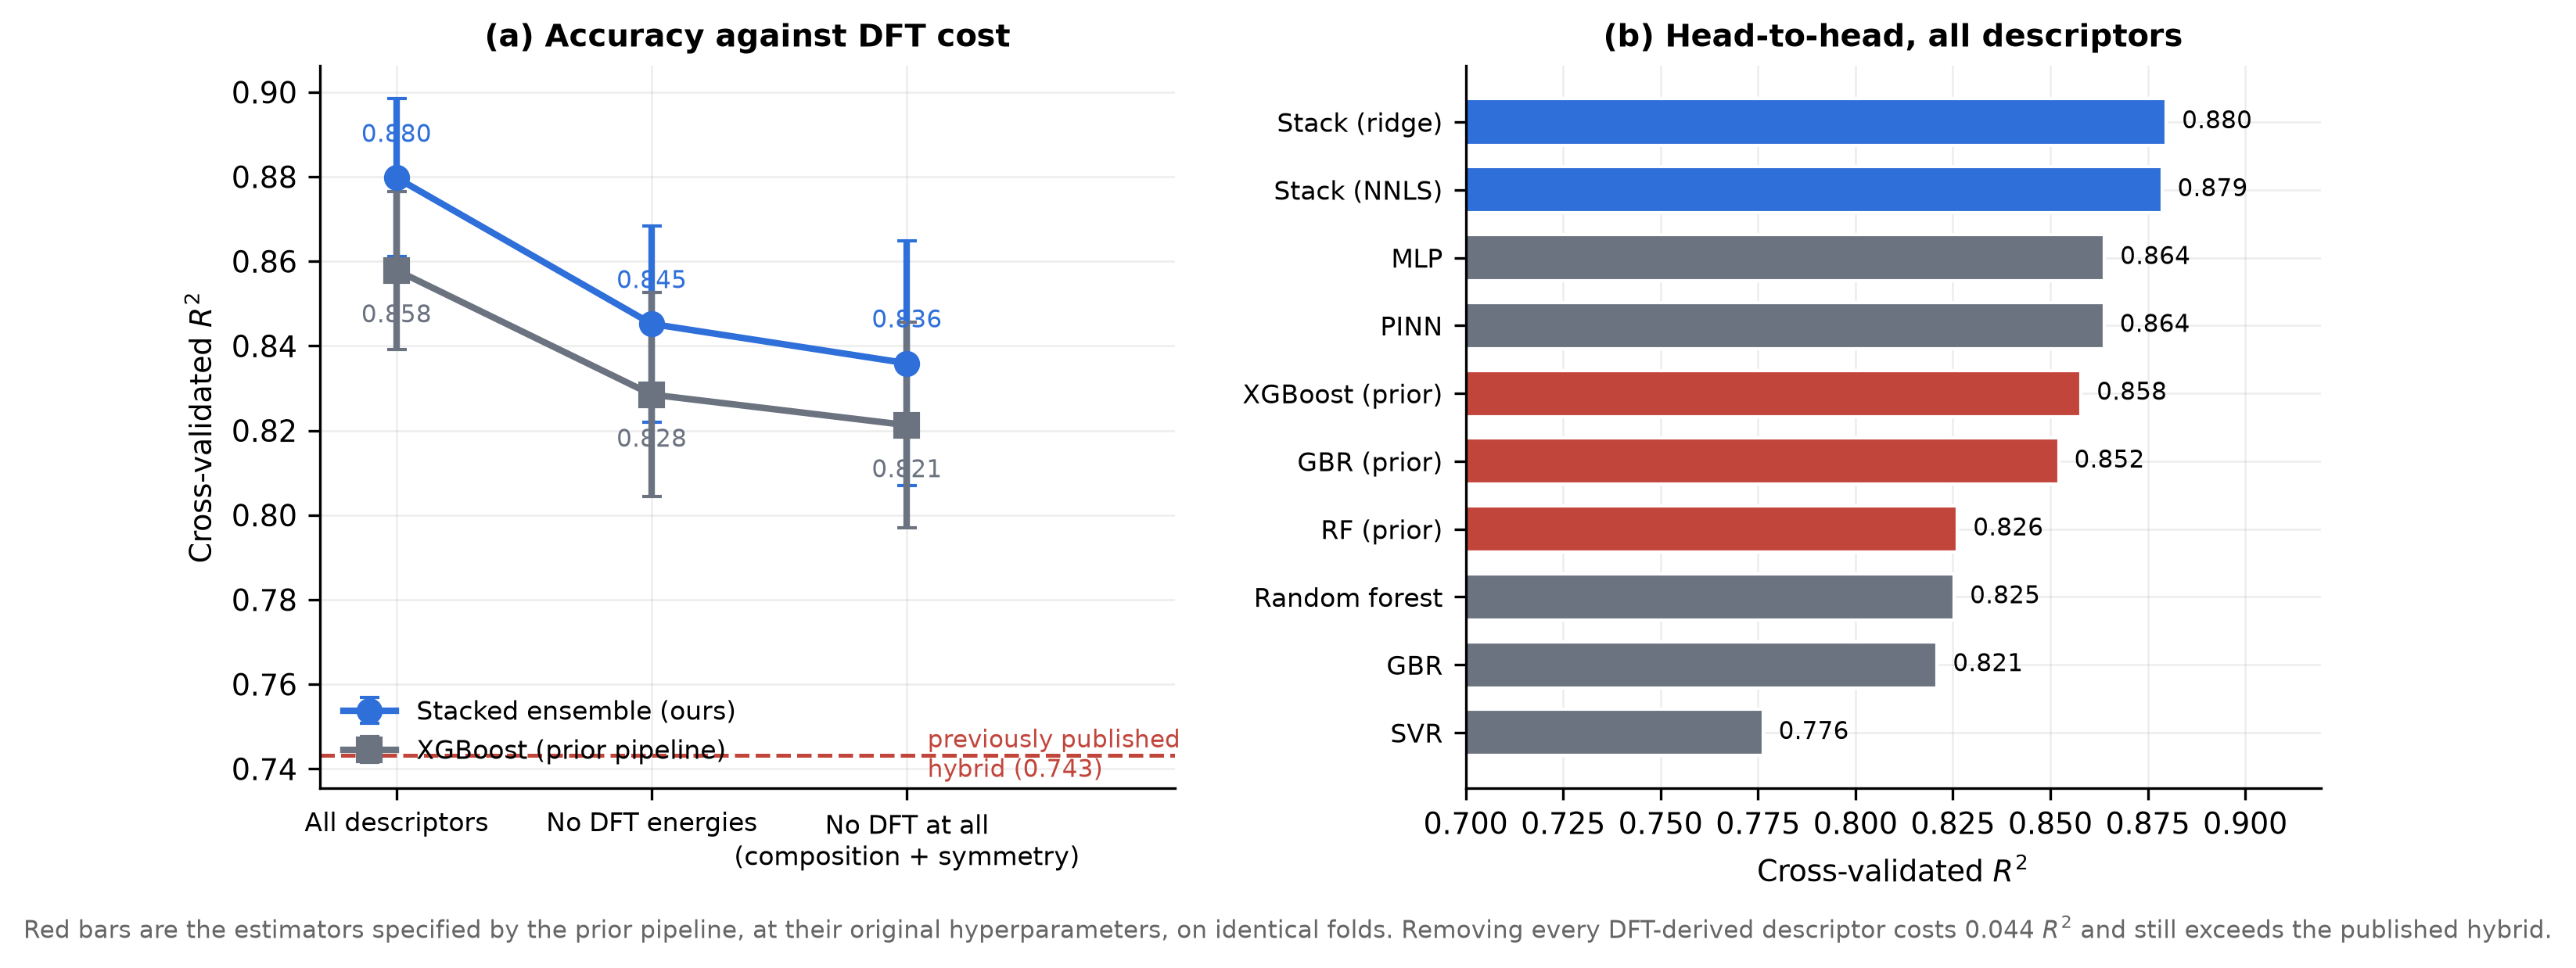
\includegraphics[width=\textwidth]{figures/fig10_feature_tiers.png}
\caption{(a) Accuracy against DFT cost. Removing every DFT-derived descriptor costs $0.044$ in $R^2$, and the resulting model still exceeds the previously published full-descriptor hybrid. (b) Head-to-head within the full tier; red bars are the estimators specified by the prior pipeline, at their original hyperparameters, on identical folds.}
\label{fig:tiers}
\end{figure*}

Removing every DFT-derived descriptor costs $0.044$ in $R^2$ and $0.057$ eV in MAE. The resulting model uses only a chemical formula and a crystal symmetry label, and it remains substantially more accurate than the previously published full-descriptor hybrid ($0.743$ / $0.555$ eV) evaluated on the same materials. This is the result with the clearest practical consequence: candidate 2D compositions can be ranked before any electronic-structure calculation is performed on them.

Fig.~\ref{fig:parity} shows the pooled out-of-fold agreement with the HSE06 reference and the regression error characteristic, which reports the fraction of materials resolved within a given absolute tolerance.

\begin{figure*}[!t]
\centering
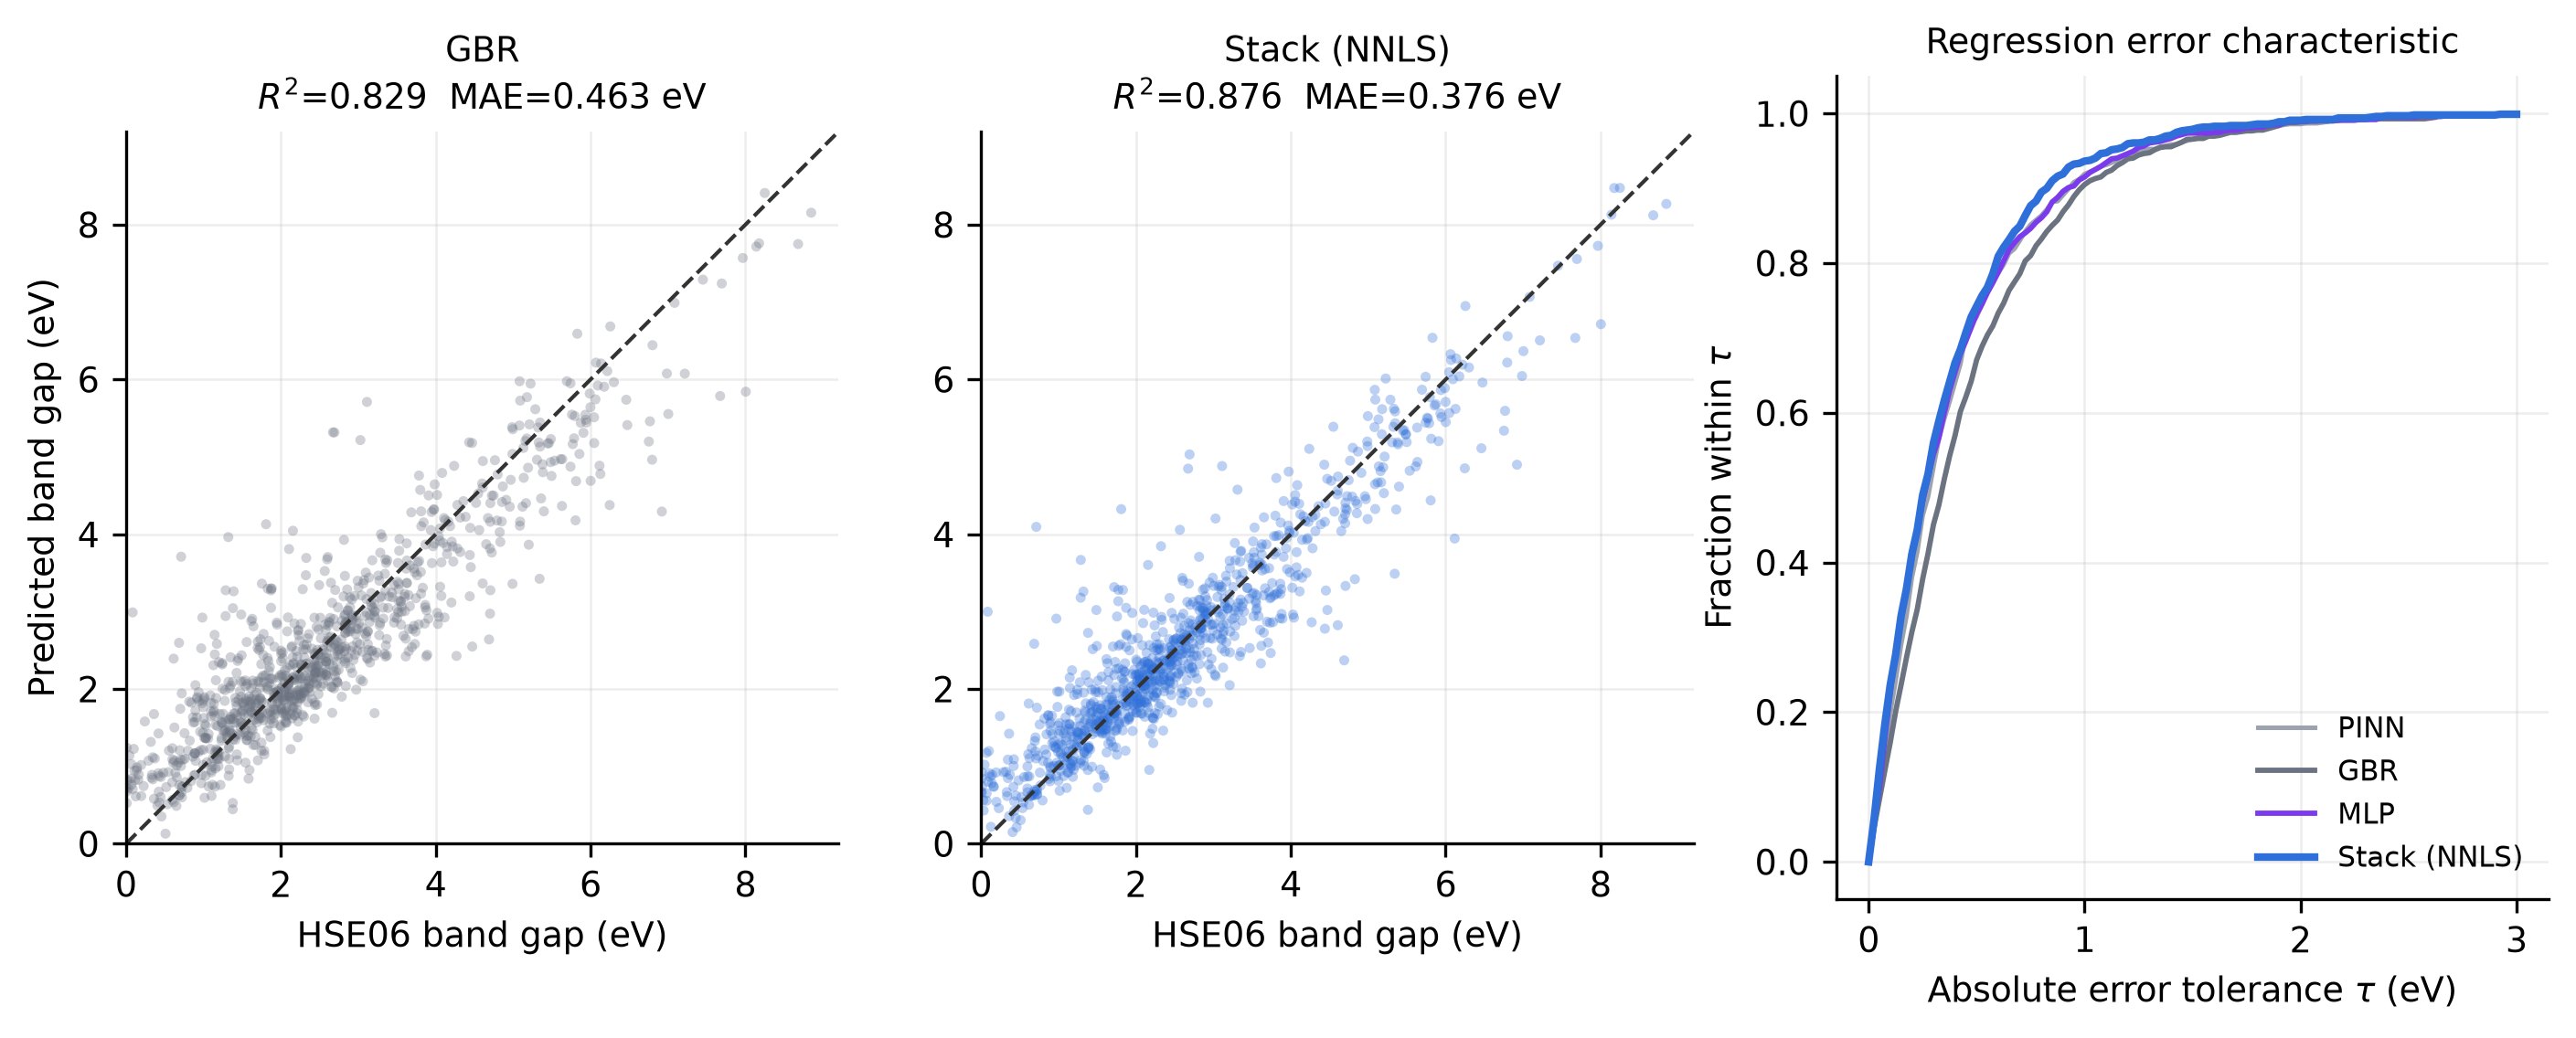
\includegraphics[width=\textwidth]{figures/fig5_parity_rec.png}
\caption{Left and centre: pooled out-of-fold predictions against HSE06 reference values for the gradient-boosting baseline and the stacked ensemble. Right: regression error characteristic curves, giving the fraction of materials predicted within a given absolute tolerance $\tau$.}
\label{fig:parity}
\end{figure*}

Fig.~\ref{fig:tiers}(b) gives the head-to-head against the prior pipeline within the full tier. The ensemble beats XGBoost on 14 of 15 fold estimates ($p = 0.025$), gradient boosting on 14 of 15 ($p = 0.002$), and random forest on 15 of 15 ($p < 0.001$). Within the DFT-free tier the margin over XGBoost narrows and is not significant ($p = 0.097$); we report this as a limitation rather than as support.

Fig.~\ref{fig:learning} shows that the ensemble's advantage is not an artefact of sample size: it leads at every training-set size tested, and its margin over the tree baselines widens as data are added, with no sign of saturation at the full 792-material training partition.

\begin{figure}[!t]
\centering
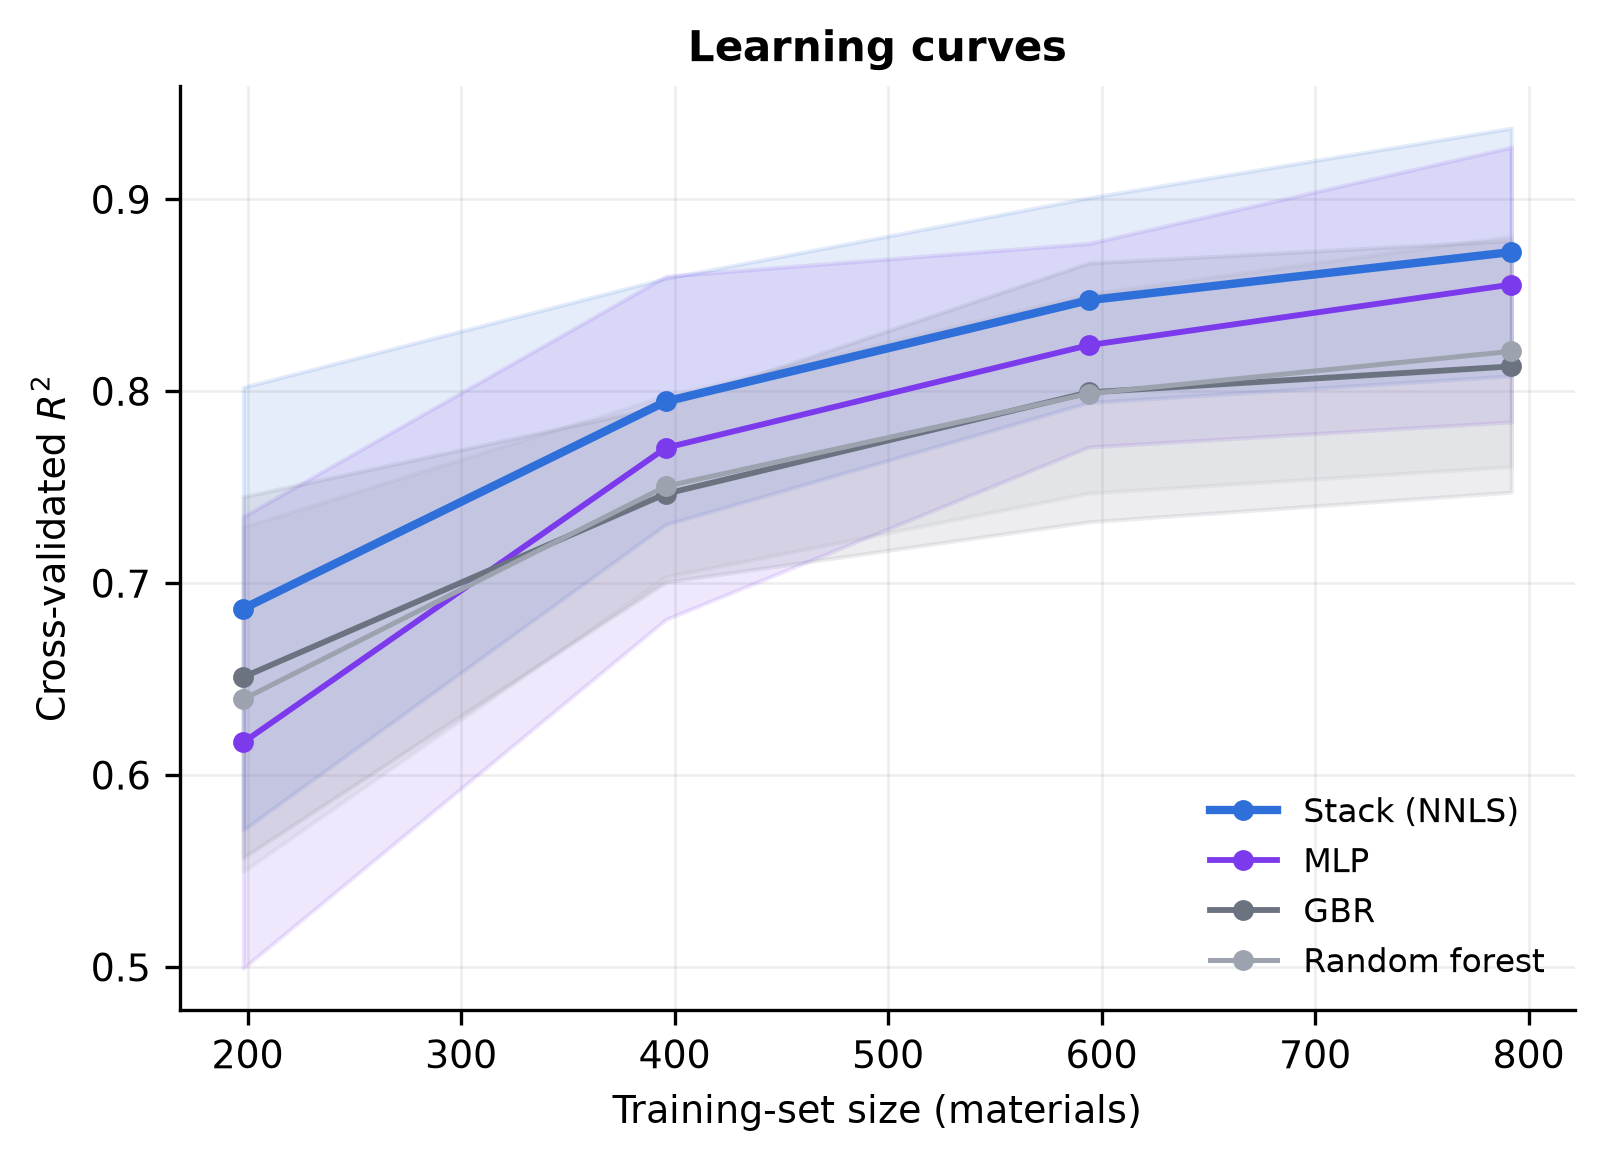
\includegraphics[width=\columnwidth]{figures/fig4_learning_curve.png}
\caption{Learning curves under grouped cross-validation. Shaded bands are 95\% confidence intervals over folds.}
\label{fig:learning}
\end{figure}

\subsection{Model Comparison}
Table~\ref{tab:benchmark} reports all models over 25 fold estimates.

\begin{table*}[!t]
\caption{Repeated grouped five-fold cross-validation, all descriptors, 25 fold estimates. ``Folds'' counts estimates beating the GBR baseline; $p$-values are Nadeau--Bengio corrected, one-sided.\label{tab:benchmark}}
\centering
\begin{tabular}{lcccc}
\toprule
Model & $R^2$ & MAE [eV] & Folds & $p$ \\
\midrule
Stacked ensemble (ridge) & $\mathbf{0.877 \pm 0.038}$ & $\mathbf{0.363}$ & 25/25 & $<0.001$ \\
Stacked ensemble (NNLS)  & $0.875 \pm 0.038$ & $0.364$ & 25/25 & $<0.001$ \\
Deep MLP                 & $0.864 \pm 0.039$ & $0.378$ & 24/25 & $0.002$ \\
Standalone PINN          & $0.856 \pm 0.043$ & $0.385$ & 22/25 & $0.033$ \\
Random forest            & $0.827 \pm 0.041$ & $0.442$ & 13/25 & $0.323$ \\
GBR (baseline)           & $0.823 \pm 0.043$ & $0.464$ & ---   & ---    \\
Hybrid GBR + corrector   & $0.810 \pm 0.047$ & $0.445$ & 12/25 & $0.271$ \\
SVR                      & $0.774 \pm 0.039$ & $0.497$ &  1/25 & --- \\
Hybrid + shrinkage gate  & $0.681 \pm 0.237$ & $0.571$ &  3/25 & $0.090$ \\
\bottomrule
\end{tabular}
\end{table*}

\begin{figure}[!t]
\centering
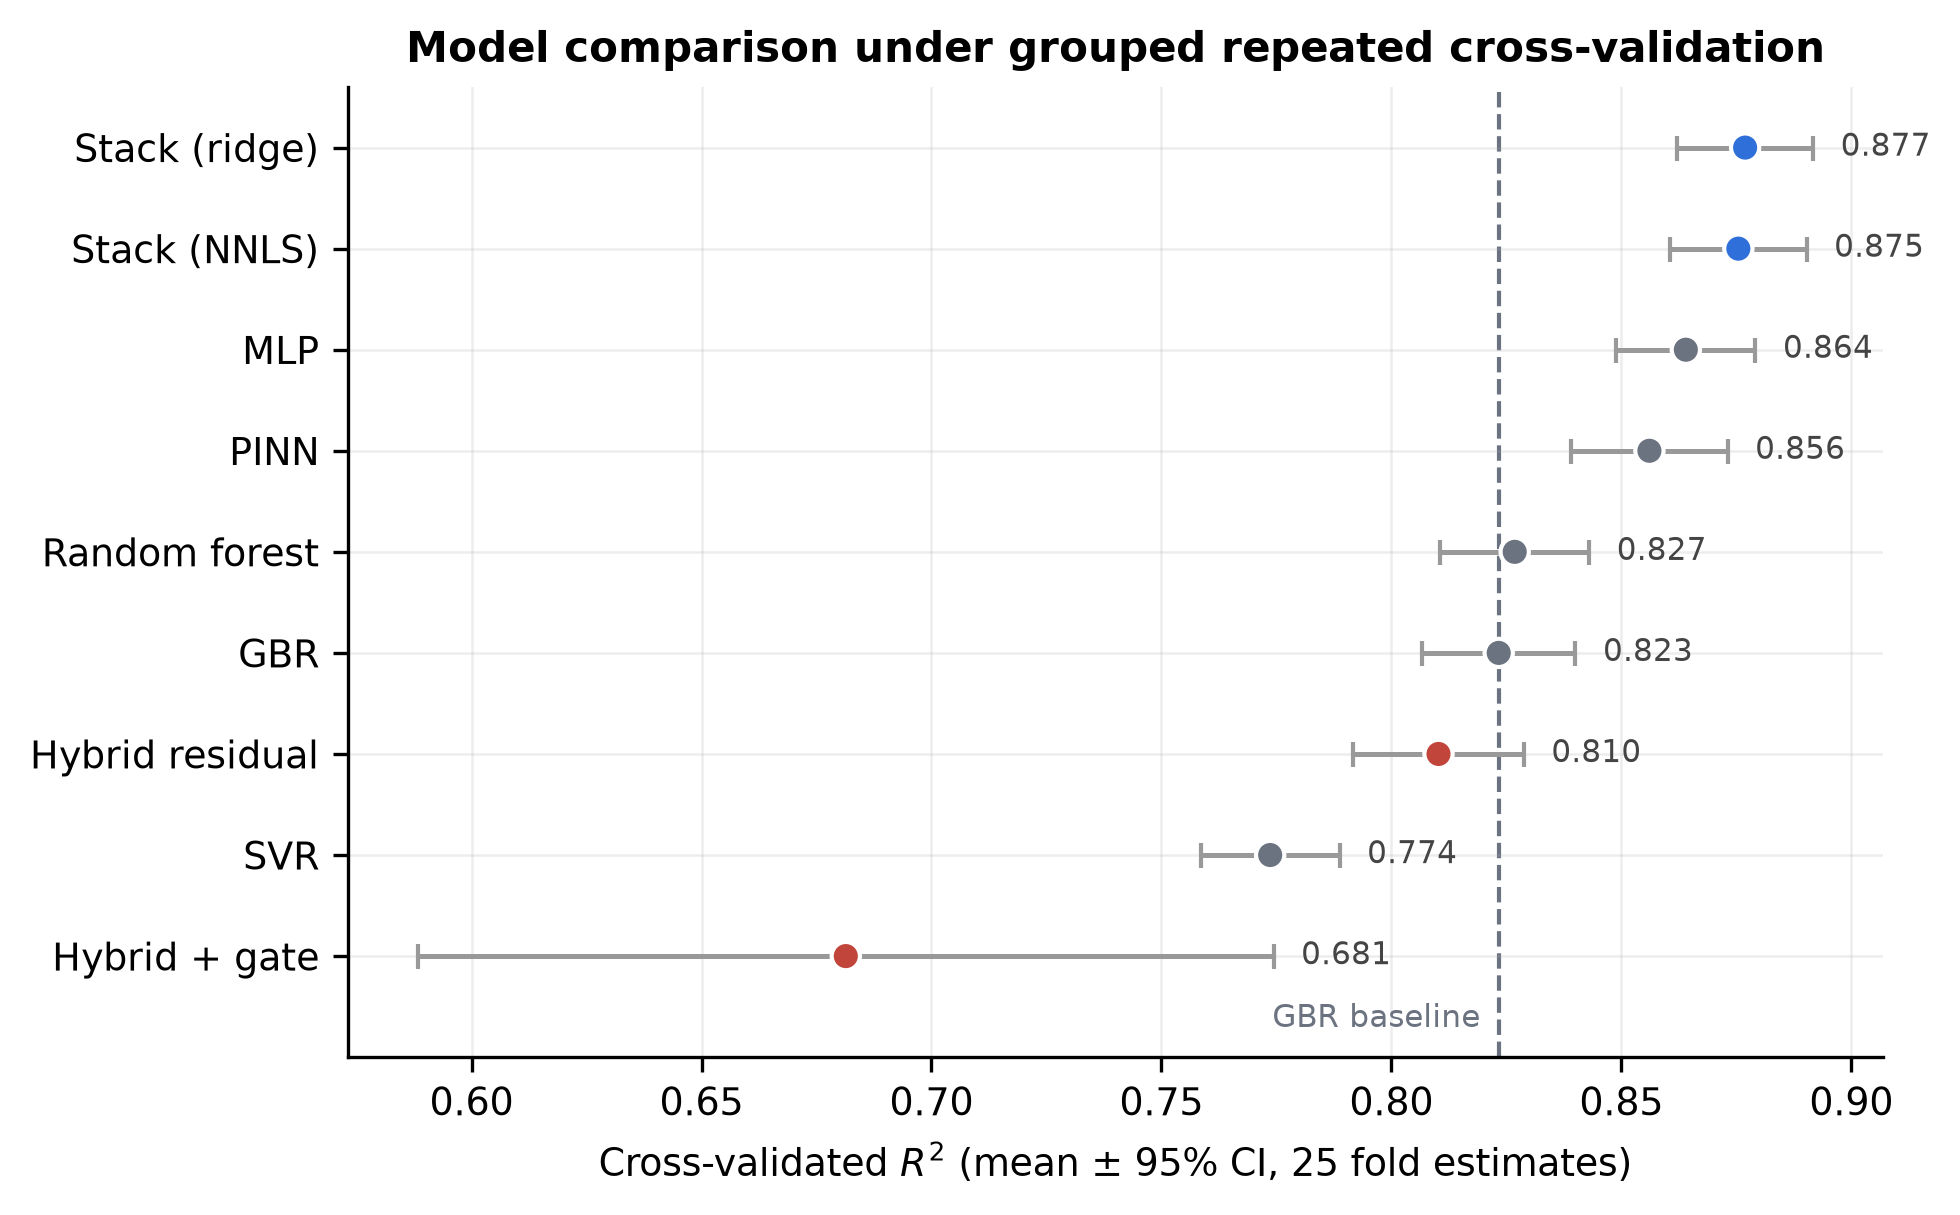
\includegraphics[width=\columnwidth]{figures/fig1_model_comparison.png}
\caption{Cross-validated $R^2$ with 95\% confidence intervals over 25 fold estimates. Hybrid variants are shown in red.}
\label{fig:comparison}
\end{figure}

Both neural models outperform every tree ensemble. With identifier-like features removed and composition statistics supplied, this task falls outside the regime in which boosted trees dominate neural networks \cite{shwartzziv2022tabular,grinsztajn2022why,mcelfresh2023when}.

Across eight independent held-out sets the ordering is reproduced: stacked ridge $0.879 \pm 0.025$, PINN $0.866 \pm 0.028$, MLP $0.858 \pm 0.032$, GBR $0.823 \pm 0.025$. The ensemble beats GBR on 8 of 8 splits ($p = 0.001$) and the MLP on 8 of 8 ($p = 0.041$); its margin over the PINN is positive on 7 of 8 splits but only marginally significant ($p = 0.051$). Per-split results are shown in Fig.~\ref{fig:holdout}. We report eight sets rather than one because a single split of this size cannot resolve closely matched models: on one 179-material split the ensemble and the PINN were indistinguishable ($0.856$ against $0.855$), a null that reflects the resolution of that split rather than equivalence of the models.

\begin{figure}[!t]
\centering
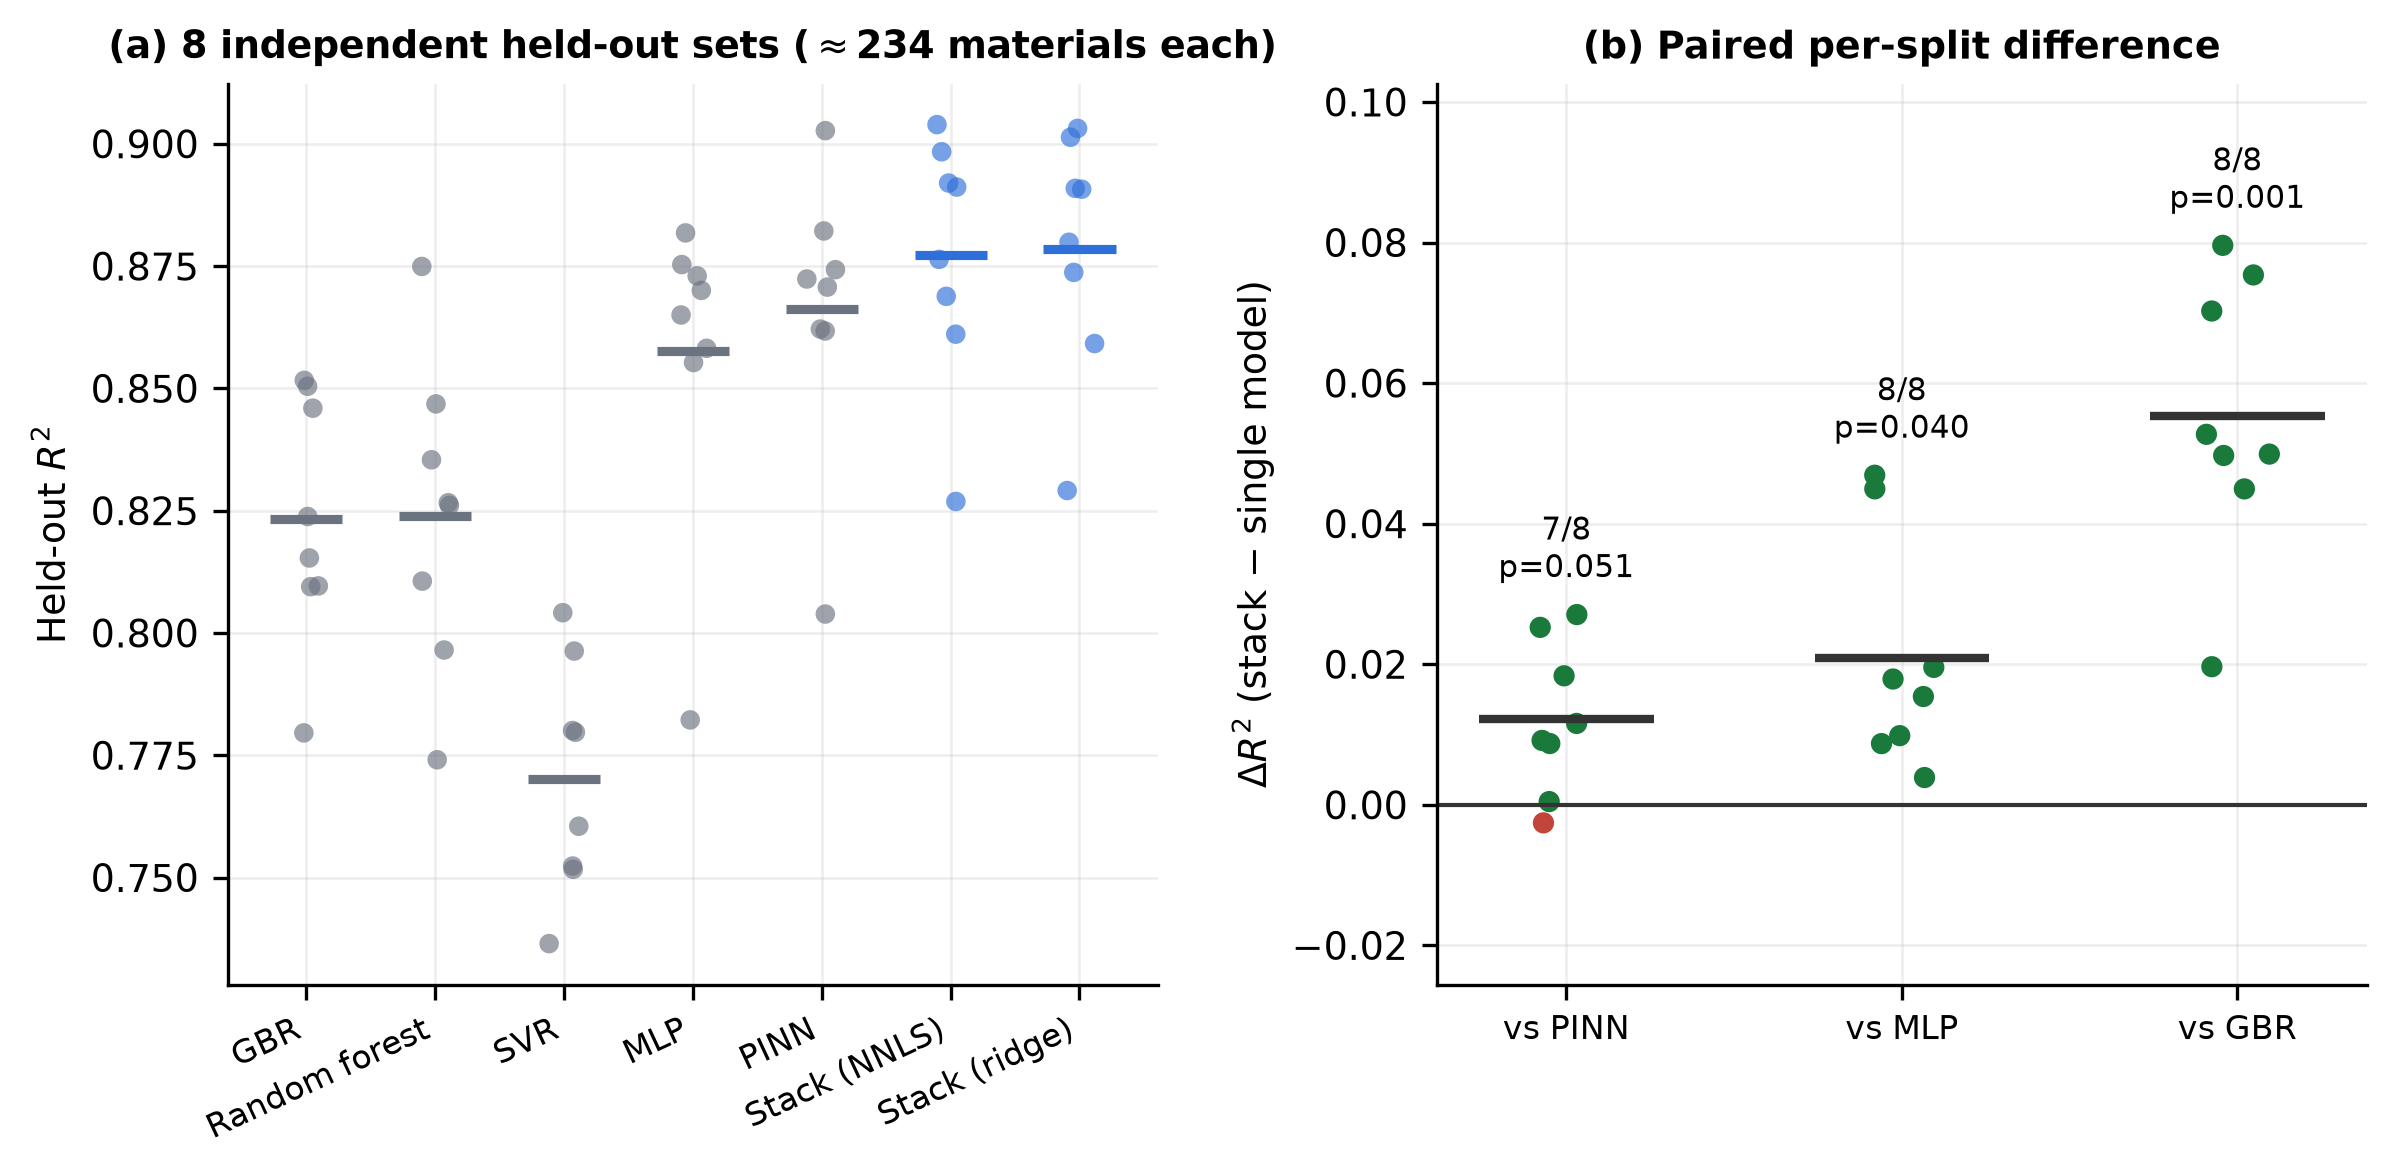
\includegraphics[width=\columnwidth]{figures/fig8_repeated_holdout.png}
\caption{Repeated held-out evaluation. (a) Per-split $R^2$ on eight independent formula-grouped held-out sets; horizontal bars are means. (b) Paired per-split difference between the stacked ensemble and each single model, annotated with splits won and the one-sided $p$-value.}
\label{fig:holdout}
\end{figure}

\subsection{The Hybrid Does Not Improve on Its Prior}
\label{sec:hybrid}
The hybrid is superior to its own gradient-boosted prior on 12 of 25 fold estimates, and the corrected test does not reject the null ($p = 0.27$). Table~\ref{tab:ablation} reports the component ablation; every configuration listed was trained and evaluated.

\begin{table}[!t]
\caption{Component ablation of the hybrid, pooled out-of-fold $R^2$.\label{tab:ablation}}
\centering
\begin{tabular}{lcc}
\toprule
Configuration & $R^2$ & $\Delta$ vs.\ full \\
\midrule
Tree prior alone, no corrector & 0.819 & $+0.018$ \\
In-sample prior (leaky)        & 0.817 & $+0.015$ \\
Without boundary penalty       & 0.806 & $+0.004$ \\
Without structural layer       & 0.804 & $+0.002$ \\
Without anisotropy penalty     & 0.804 & $+0.002$ \\
\textbf{Full framework}        & 0.801 & --- \\
Without quantile heads         & 0.796 & $-0.005$ \\
Without residual head          & 0.766 & $-0.035$ \\
\bottomrule
\end{tabular}
\end{table}

\begin{figure}[!t]
\centering
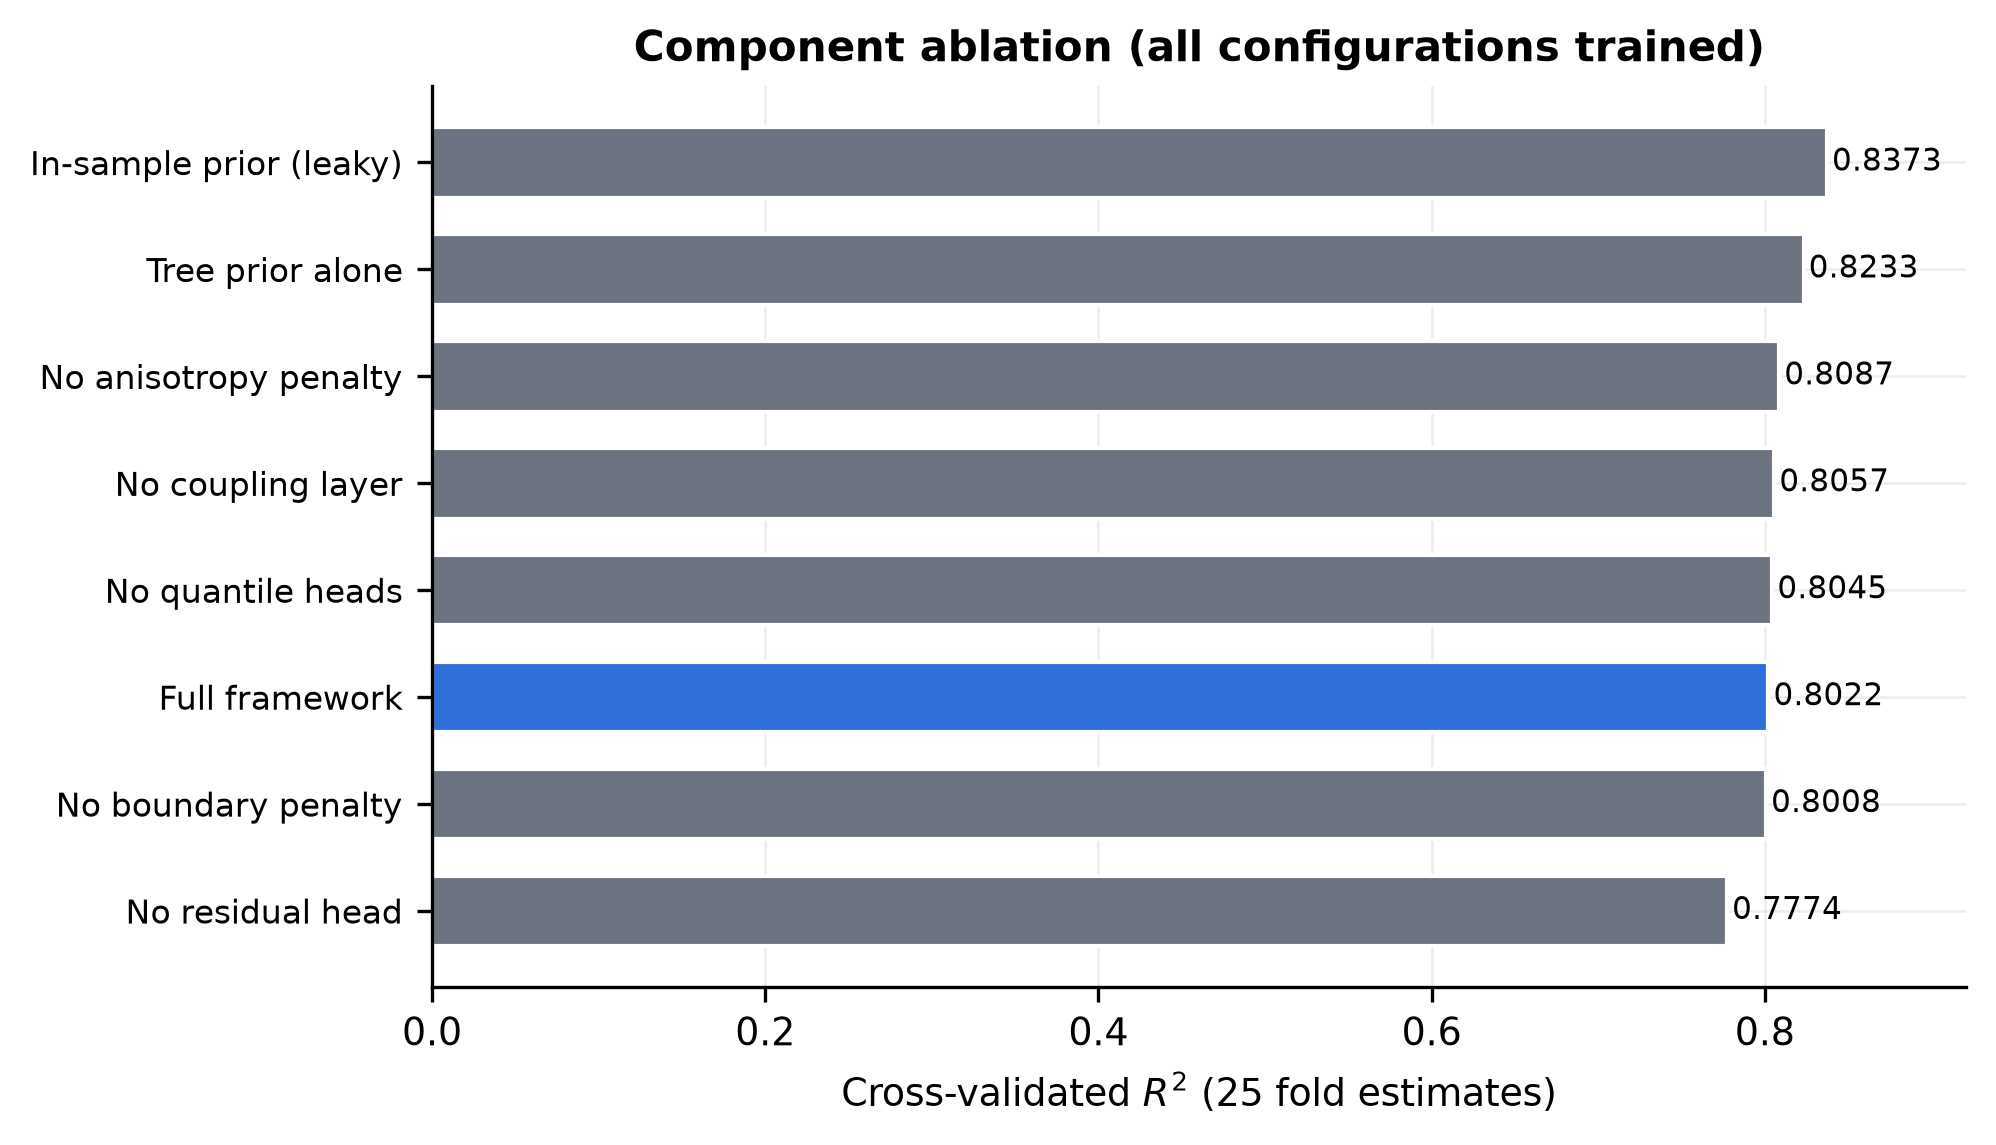
\includegraphics[width=\columnwidth]{figures/fig6_ablation.png}
\caption{Component ablation of the hybrid. Every configuration shown was trained and evaluated; no physics-motivated component contributes positively, and the tree prior alone is the strongest configuration.}
\label{fig:ablation}
\end{figure}

No physics-motivated component contributes positively, and the tree prior alone is the strongest configuration in the table (Fig.~\ref{fig:ablation}). The second row identifies the mechanism: reverting to an in-sample prior \emph{raises} measured $R^2$. With a prior that appears near-perfect on training rows, the correction head has almost no residual signal to fit; it learns to emit approximately zero and degenerates into a pass-through of the tree. The previously reported gain is therefore substantially an artefact of the corrector being trained to be inert, and the ablation recovers that artefact on demand by changing one line.

We also tested the natural remedy. A shrinkage gate constrains the correction by $\sigma(\cdot) \in (0,1)$, initialised near zero so the model begins as a pass-through and must earn any departure. It did not work: the gate converged small ($0.081 \pm 0.007$) but accuracy destabilised ($R^2 = 0.681 \pm 0.237$, with 7 of 25 fold estimates below $0.70$ and one at $-0.24$). Shrinking the gate rescales the gradient reaching the head, whose raw output grows to compensate, leaving the product poorly controlled on unseen data.

\subsection{Uncertainty Calibration}
The hybrid predicts quantiles at $\tau \in \{0.25, 0.50, 0.75\}$, previously described as uncertainty estimates. Empirical coverage of the predicted interval,
\begin{equation}
C = \frac{1}{N}\sum_{i=1}^{N}
  \mathbb{1}\!\left[q_{0.25,i} \leq y_i \leq q_{0.75,i}\right],
\label{eq:coverage}
\end{equation}
should equal the nominal level of $0.50$; the measured value is $C = 0.172$ at a mean interval width of $2.47$ eV (Fig.~\ref{fig:calibration}). The intervals are simultaneously wide and badly miscalibrated, and the deficit persists across every nominal level tested (Fig.~\ref{fig:calibration}(a)). We therefore withdraw the uncertainty claim; supporting one requires scoring the predictive distribution with a proper rule \cite{gneiting2007probabilistic}.

\begin{figure}[!t]
\centering
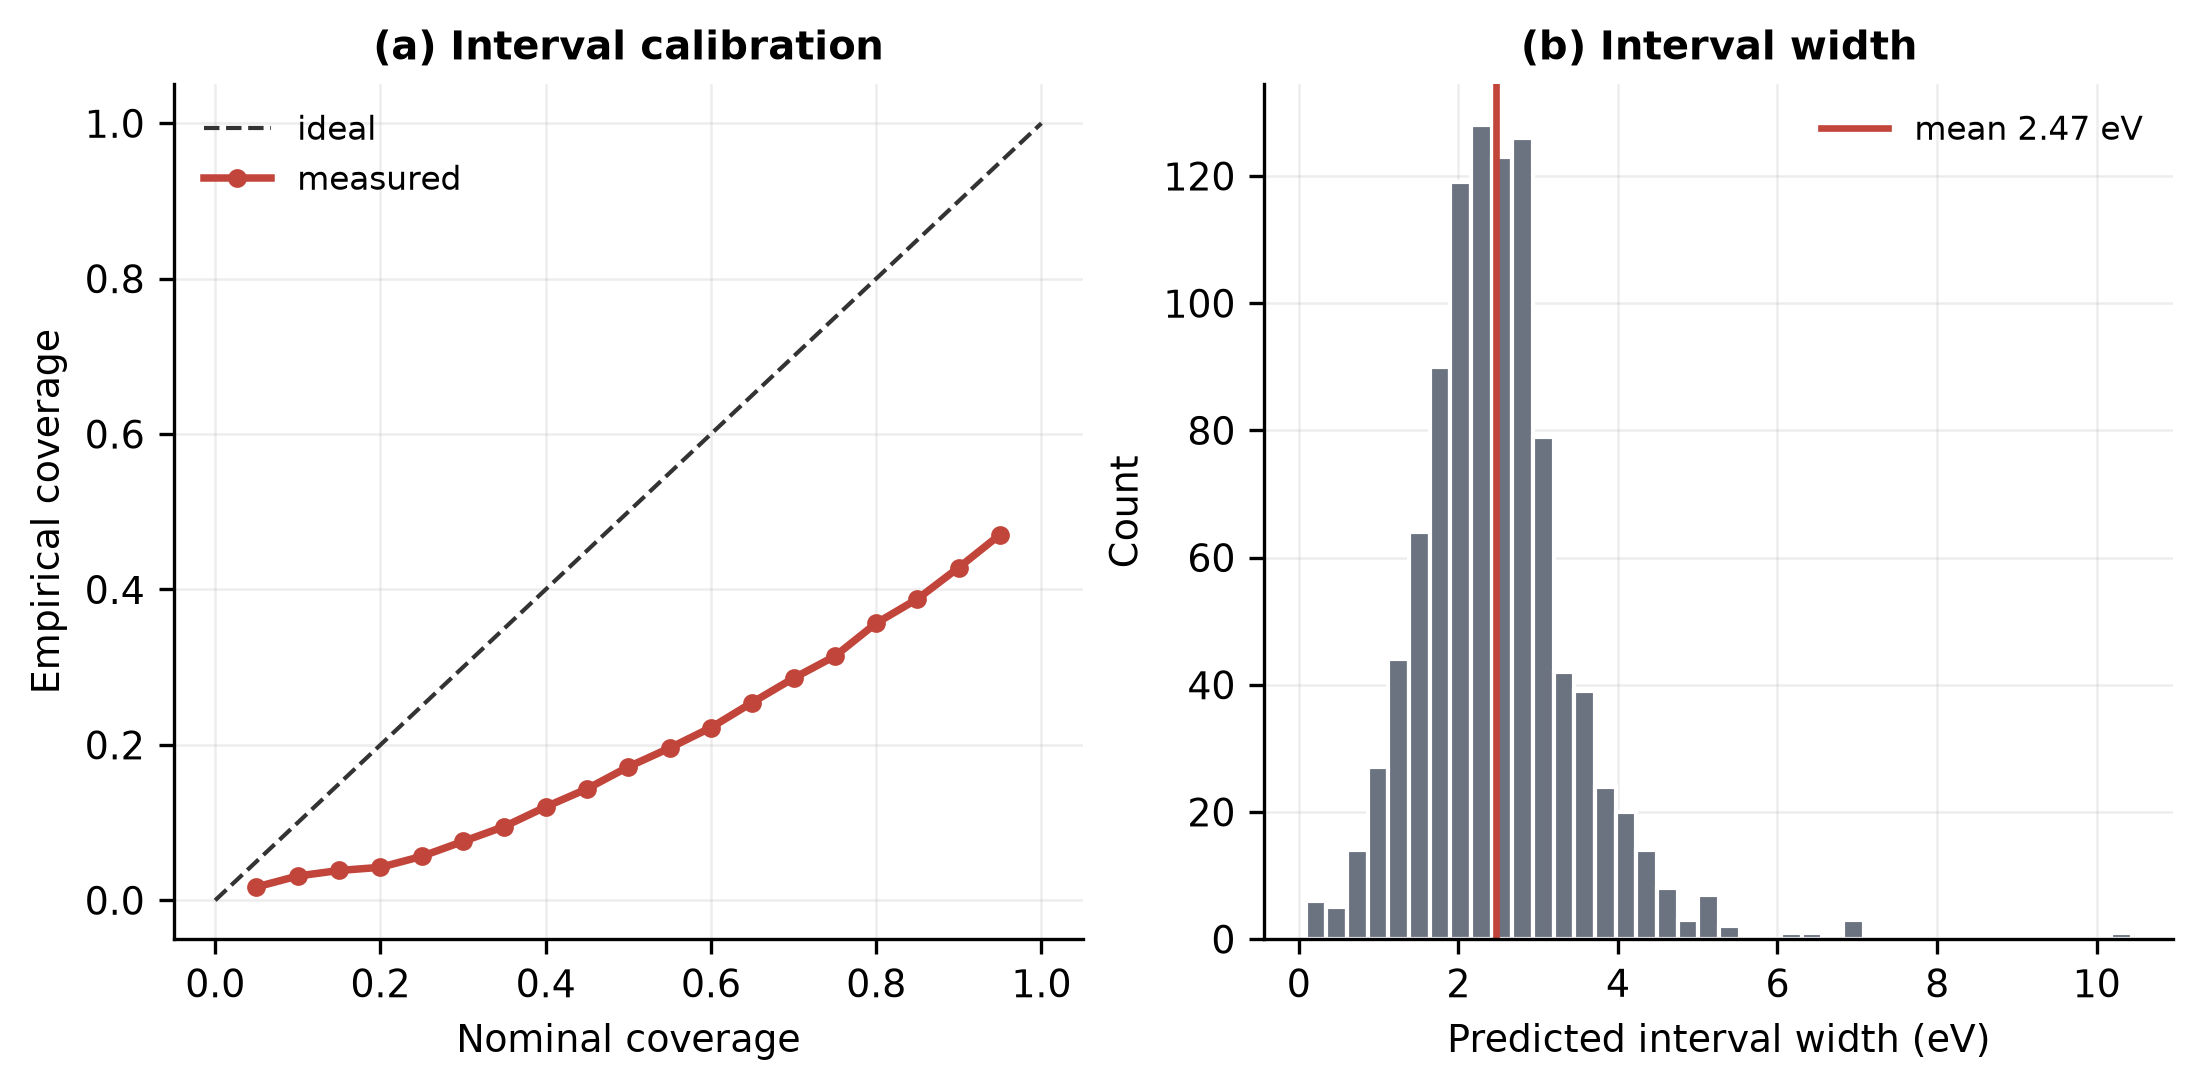
\includegraphics[width=\columnwidth]{figures/fig7_calibration.png}
\caption{Quantile calibration of the hybrid. (a) Empirical against nominal coverage; the model is over-confident at every level. (b) Distribution of predicted interval widths.}
\label{fig:calibration}
\end{figure}

\subsection{Why the Ensemble Is Worth Its Cost}
\label{sec:utility}
The ensemble's margin over the best single model is small ($\Delta R^2 \approx 0.016$) and would not by itself justify a fivefold training cost. We therefore evaluate it on three decision-relevant axes (Fig.~\ref{fig:utility}).

\begin{figure*}[!t]
\centering
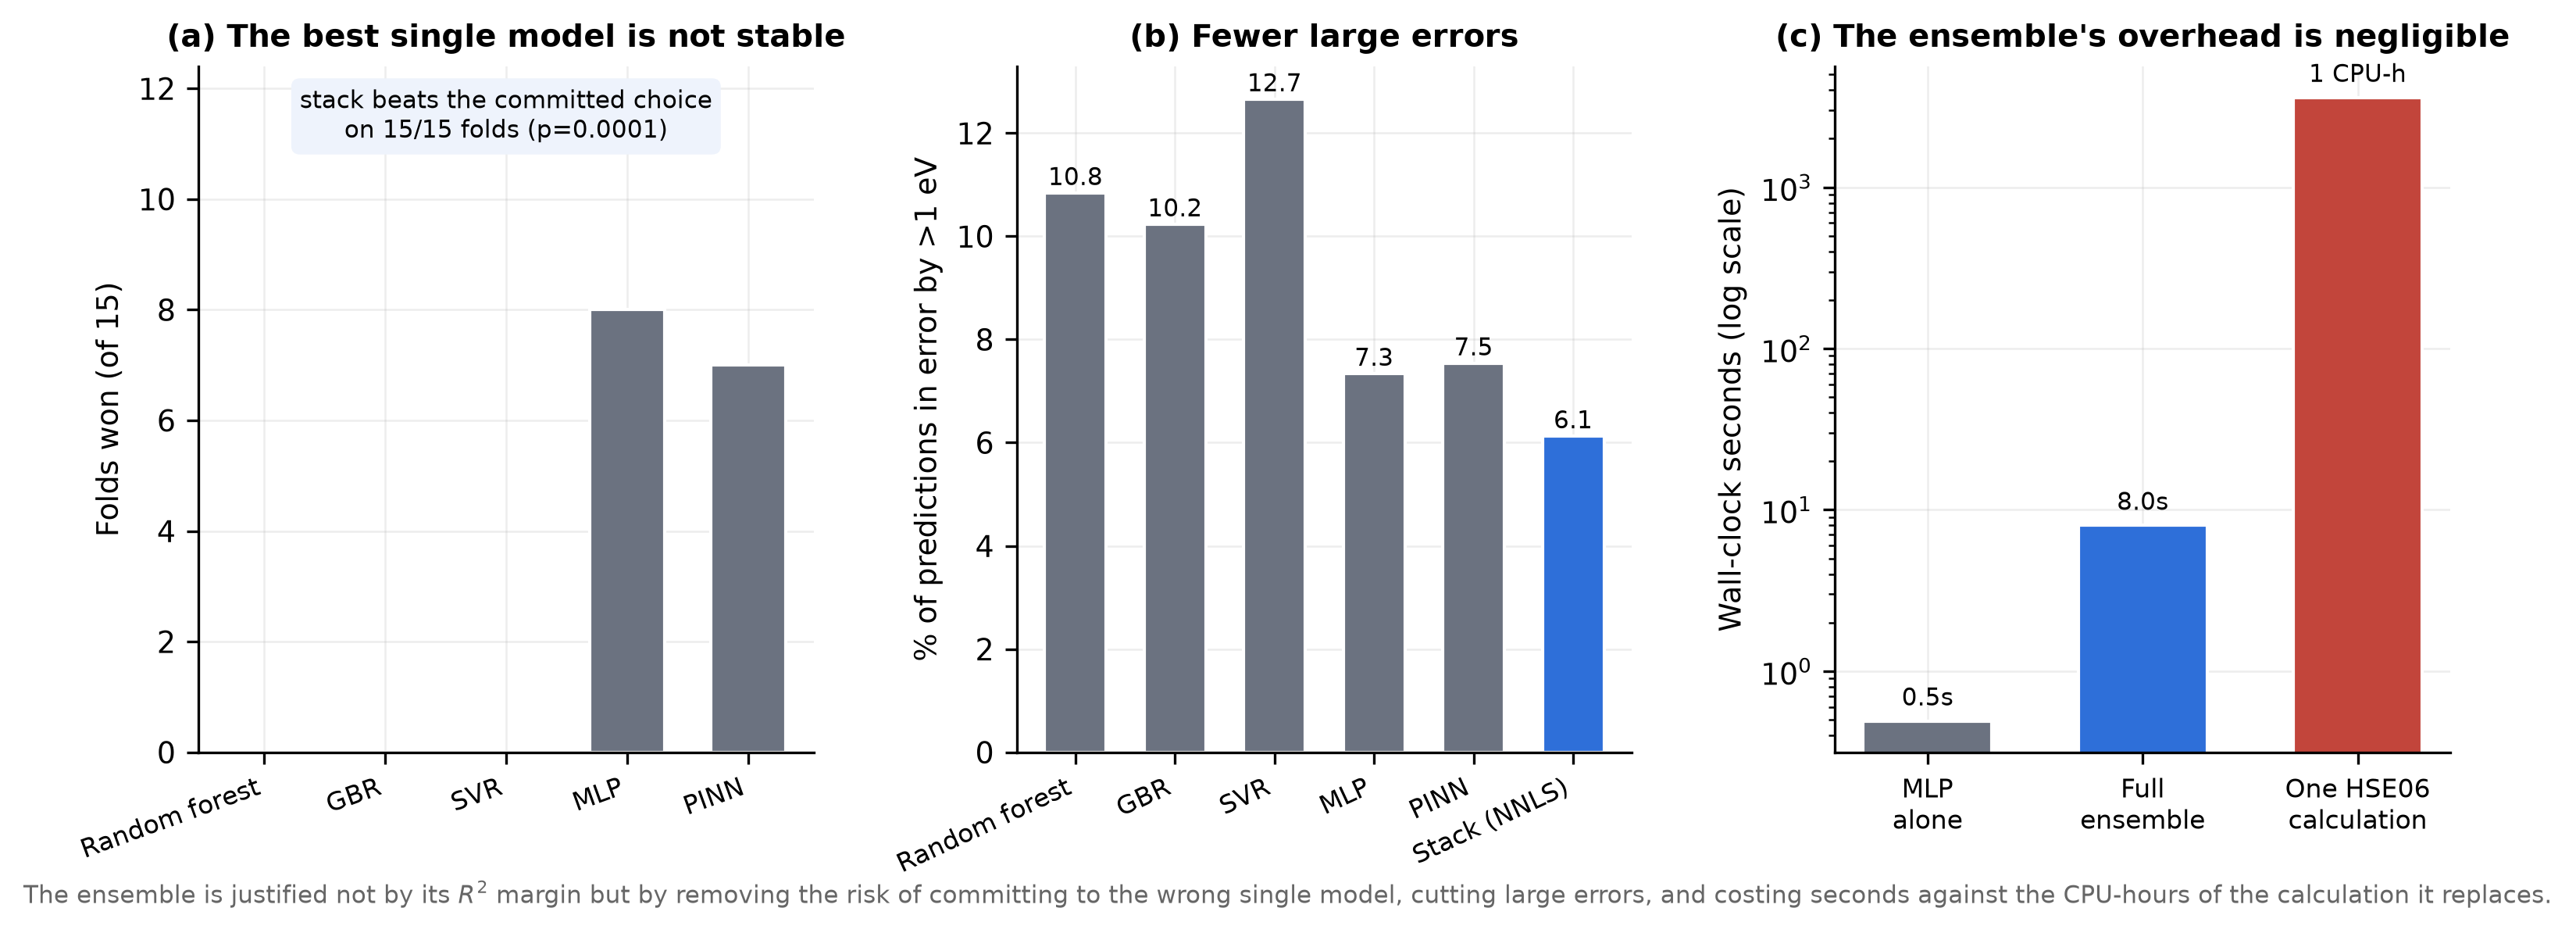
\includegraphics[width=\textwidth]{figures/fig9_utility.png}
\caption{(a) The best single model is unstable across folds. (b) Rate of predictions in error by more than 1 eV. (c) Measured training cost against the calculation being replaced, on a logarithmic scale.}
\label{fig:utility}
\end{figure*}

\textit{Model-selection risk.} The best single model is not the same model on every fold: the MLP wins 8 of 15 and the PINN 7, and no tree model ever wins. A practitioner must commit to one architecture in advance, and cannot know which. The ensemble beats the best-on-average committed choice on 15 of 15 folds ($p = 0.0001$), and its regret against a per-fold oracle is negative ($-0.008$) --- it outperforms an oracle that always selects the best single model. Committing instead to the weakest plausible choice costs $0.102$ in $R^2$, roughly six times the ensemble's margin over the strongest.

\textit{Large-error rate.} Screening is harmed more by rare large errors, which move a material between application classes, than by average error. Predictions in error by more than 1 eV occur at $6.1\%$ for the ensemble against $7.3\%$ for the best single model and $10$--$13\%$ for the tree baselines; the 95th-percentile absolute error is $1.10$ eV against $1.18$ eV.

\textit{Cost.} Training the full ensemble, including the out-of-fold predictions the meta-learner requires, takes $8.0$ s against $0.5$ s for the MLP alone, and inference over 198 materials takes $22$ ms. The relative overhead of $16\times$ is real but the absolute cost is eight seconds, against the CPU-hours of the HSE06 calculation being replaced. The standard objection that an ensemble of $N$ models costs $N$ times more \cite{tavazza2023approaches} does not bind in this regime.

We report one axis that does not support the ensemble. On a screening task measuring wasted DFT evaluations per true hit, results are mixed: the ensemble is best for a visible-photocatalysis window ($1.8$--$3.0$ eV), the PINN is best for a photovoltaic window ($1.0$--$2.0$ eV), and several models tie for wide-gap selection.

\section{Discussion}
\label{sec:discussion}

\subsection{Why Residual Correction Fails}
Once the prior is constructed out of fold, its residuals on unseen materials are dominated by irreducible noise rather than recoverable structure, and a corrector fitted to them adds variance without removing bias. This is not specific to materials data; residual-boosting correctors are known to yield negative gains when the residual signal is noise-dominated \cite{airlangga2025hybrid}. The practical consequence is that hybrid residual designs must be validated against their own prior with an out-of-fold construction. Compared against an in-sample prior they can appear to help while doing nothing, and that appearance is stable enough to survive review.

\subsection{What the Ensemble Buys}
The stacking gain arises from error diversity rather than from any member's individual strength. The mean pairwise correlation between base-learner residuals is $0.750$, and Fig.~\ref{fig:correlation} shows the neural and tree models forming visibly distinct error clusters; it is combination across those clusters that the meta-learner exploits.

\begin{figure}[!t]
\centering
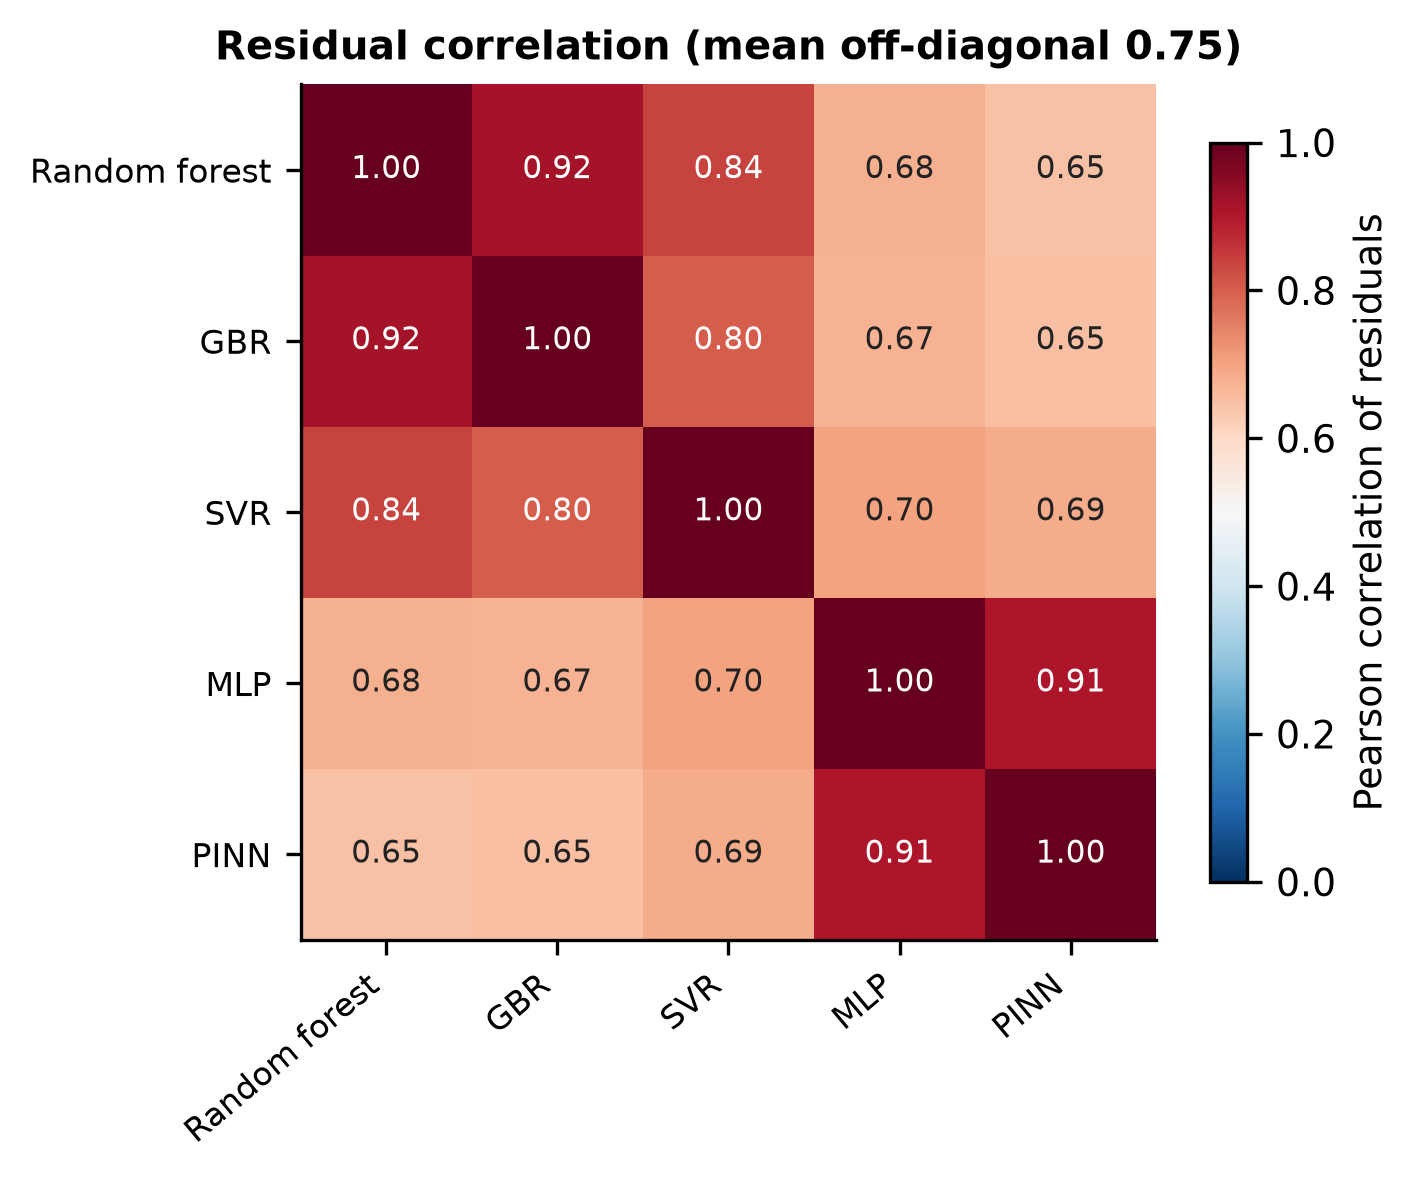
\includegraphics[width=\columnwidth]{figures/fig3_error_correlation.png}
\caption{Pearson correlation between out-of-fold residuals of the base learners. Lower correlation between clusters is what makes stacking profitable.}
\label{fig:correlation}
\end{figure}

Fig.~\ref{fig:contributions} contrasts the fitted ensemble weights with a drop-one ablation. The two disagree: SVR receives zero weight yet gradient boosting receives $0.238$ while contributing nothing measurable when removed. Collinear members split weight between them, so weights alone cannot establish a contribution and the drop-one test is the appropriate instrument. That test orders the members consistently with their individual accuracy, but no single member's contribution is statistically significant once the Nadeau--Bengio correction is applied ($p = 0.11$--$0.45$); the uncorrected test would report $p < 0.05$ for three of them. The defensible statement is that the ensemble as a whole outperforms its members, not that any one member is indispensable.

\begin{figure}[!t]
\centering
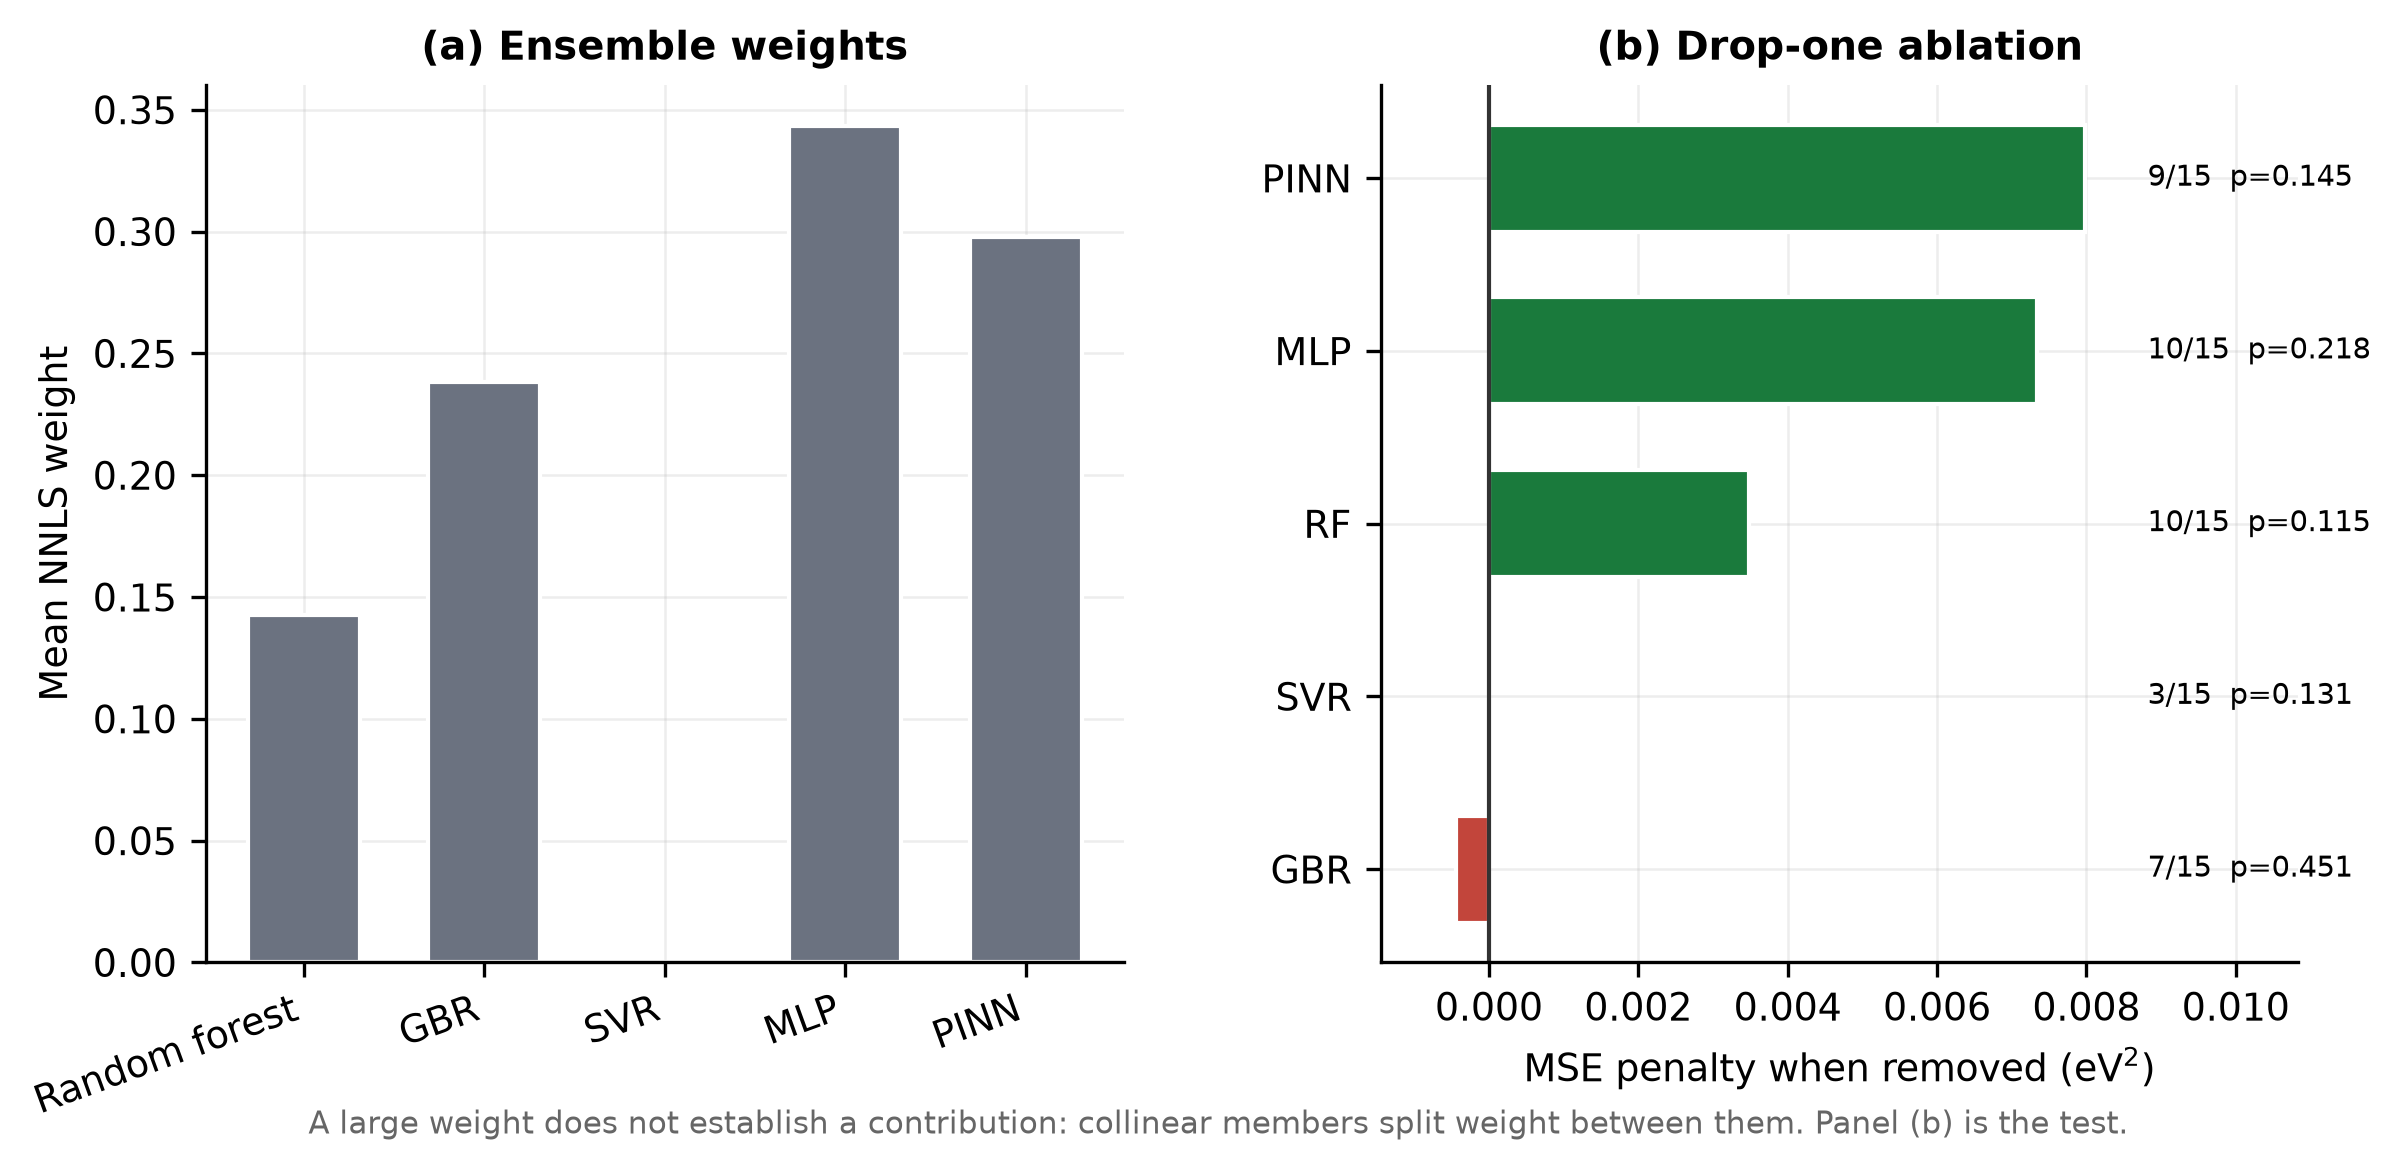
\includegraphics[width=\columnwidth]{figures/fig2_ensemble_contributions.png}
\caption{Ensemble member contributions. (a) Mean non-negative stacking weights. (b) Drop-one ablation: change in ensemble MSE when each member is removed, with fold estimates degraded and the corrected one-sided $p$-value. Positive values indicate that removing the member hurts.}
\label{fig:contributions}
\end{figure}

\subsection{On the Anisotropy Hypothesis}
Our results do not refute the physical hypothesis that motivated the original architecture --- that in-plane anisotropy shapes band gaps in rectangular 2D lattices \cite{rodin2014strain,tran2014layer,kim2015observation}. They show that the present implementation cannot test it: the coupling layer was wired to two formation energies, and the available data contain no in-plane lattice vectors. Recovering $a$ and $b$ from a full C2DB structure pull is the single most valuable extension of this work.

\subsection{Limitations}
All data derive from one database and one Bravais class, with 1{,}169 labelled materials. In the DFT-free tier the ensemble's advantage over a well-tuned XGBoost is not statistically significant. We compare against tabular baselines only, not against structure-aware graph networks \cite{xie2018crystal,schutt2018schnet,chen2019graph,choudhary2021atomistic,chen2022universal}, which require relaxed atomic coordinates --- and which, we note, would reintroduce exactly the DFT dependence the DFT-free tier is designed to avoid.

\section{Conclusion}
\label{sec:conclusion}
Band gaps of rectangular-lattice two-dimensional materials can be predicted to $R^2 = 0.836$ and MAE $0.417$ eV from chemical composition and crystal symmetry alone, with no electronic-structure calculation on the target material. That model is more accurate than a previously published physics-informed hybrid that used the full DFT-derived descriptor set, and it is applicable to compounds that have never been calculated --- which the full-descriptor model, by construction, is not.

Under the same leakage-controlled protocol, the physics-informed hybrid residual architecture does not improve on the gradient-boosted prior it corrects, and none of its physics-motivated components contributes measurably. The previously reported improvement is reproduced on demand by reverting a single implementation detail, identifying it as an evaluation artefact rather than a modelling effect. We regard this negative result as the more transferable of the two findings, because hybrid residual designs are widely reported to help and the specific way this one appeared to help is easy to reproduce by accident.

Where a modest ensemble gain must be justified, we suggest it be justified as we have here: by the risk it removes and the errors it avoids, at a cost measured against the calculation it replaces, rather than by a difference in $R^2$.

\section*{Data and Code Availability}
All code, the curated dataset, per-fold out-of-sample predictions, and the scripts generating every table and figure are available at \url{https://github.com/adhvayjagadeesh/DFT---Machine-Learning--PINN}. Every experiment reproduces from a single command under a pinned environment with a fixed random seed.

\bibliographystyle{IEEEtran}
\bibliography{references}

\begin{IEEEbiographynophoto}{Adhvay Jagadeesh}
is a student researcher with the Aspiring Scholars Directed Research Program (ASDRP), Fremont, CA, USA. His research interests include machine learning for materials science, physics-informed neural networks, and computational modeling of two-dimensional materials.
\end{IEEEbiographynophoto}

% =====================================================================
% NOTE TO AUTHOR: IEEE Access requires a short biography for EVERY
% author. The two below are placeholders and MUST be replaced before
% submission. Use
% \begin{IEEEbiography}[{\includegraphics[width=1in,height=1.25in,clip,keepaspectratio]{photo}}]{Name}
% if you wish to include an author photograph.
% =====================================================================
\begin{IEEEbiographynophoto}{Rutvi Mudalagi}
PLACEHOLDER --- biography required before submission.
\end{IEEEbiographynophoto}

\begin{IEEEbiographynophoto}{Marx Akl}
PLACEHOLDER --- biography required before submission. Faculty advisor, Aspiring Scholars Directed Research Program (ASDRP), Fremont, CA, USA.
\end{IEEEbiographynophoto}

\EOD

\end{document}
